\chapter{Metodo Voltamperometrico}
Questo metodo serve per misurare \textbf{resistenze elettriche}:
\begin{center}
    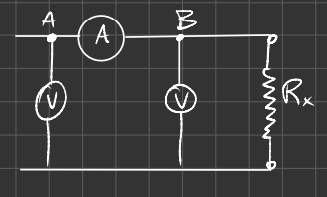
\includegraphics[width=.4\textwidth]{Images/figure2.png}
\end{center}
Per determinare $R_x$ viene alimentata in \textbf{continua} e vengono misurate \textbf{tensione} e \textbf{corrente}.\\ \\
Sono possibili due tipi di collegamenti:
\begin{itemize}
    \item \textbf{Metodo voltamperometrico a monte dell'amperometro}
    \item \textbf{Metodo voltamperometrico a valle dell'amperometro}
\end{itemize}
\section{Metodo voltamperometrico a monte dell'amperometro}
Il \textbf{voltmetro a monte} è preferibile quando si devono misurare \textbf{resistenze elevate}, ossia confrontabili con la \textbf{resistenza interna al voltmetro} $R_v$:
\begin{center}
    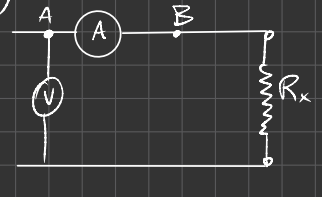
\includegraphics[width=.4\textwidth]{Images/figure3.png}
\end{center}
\begin{equation*}
\begin{dcases}
     I_x = I_m\\
    V_m = V_A + V_x
\end{dcases}
\end{equation*}
Quindi:
\begin{equation*}
    R_x = \frac{V_x}{I_x} = \frac{V_m - V_A}{I_m} = \underbrace{\frac{V_m}{I_m}}_{R_m} - R_A
\end{equation*}
Di solito $R_A$ (chiamata anche \textbf{errore di consumo}) ci viene data dal costruttore.\\ \\
\subsection{Incertezza}
\begin{equation*}
    u_{R_x} = \sqrt{u^2_{\left(\frac{V_m}{I_m}\right)} + u^2_{R_A}} 
\end{equation*}
dove:
\begin{equation*}
    u^2_{\left(\frac{V_m}{I_m}\right)} ={\left(\frac{V_m}{I_m}\right)}^2\left(\dot{u}^2_{V_m} + \dot{u}^2_{I_m} \right)
\end{equation*}
\begin{equation*}
    u_{R_A} = \frac{\Delta R_A}{\sqrt{3}}
\end{equation*}

\section{Metodo voltamperometrico a valle dell'amperometro}
Questa configurazione si utilizza per misurare \textbf{resistenze piccole} in rapporto alla \textbf{resistenza interna del voltmetro}:
\begin{center}
    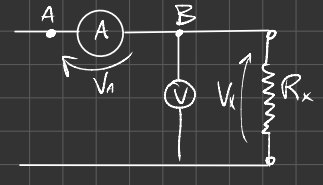
\includegraphics[width=.4\textwidth]{Images/figure4.png}
\end{center}
\begin{equation*}
    \begin{dcases}
        V_m = V_x\\
        I_m = I_x + I_v
    \end{dcases}
\end{equation*}
Quindi (lavoreremo più facilmente con le \textbf{ammettenze}):
\begin{equation*}
    G_x = \frac{I_m - I_v}{V_m} = G_m - G_v
\end{equation*}
\subsection{Incertezza}
\begin{equation*}
    u_{G_x} = \sqrt{u^2_{\left(\frac{I_m}{V_m}\right)} + u^2_{G_v}}
\end{equation*}
dove:
\begin{equation*}
   u^2_{\left(\frac{I_m}{V_m}\right)}=  \left(\frac{I_m}{V_m}\right)^2 \cdot \left(\dot{u}^2_{I_m} + \dot{u}^2_{V_m} \right)
\end{equation*}